\documentclass[a4paper,10pt]{article}
\usepackage[utf8]{inputenc}
\usepackage[T1]{fontenc}
\usepackage{mathptmx}
\usepackage{amsmath}
\usepackage{graphicx}
\usepackage{caption}
\usepackage{float}
\usepackage{booktabs}
\usepackage{tabularx}
\usepackage{multirow}
\usepackage{enumitem}
\usepackage{url}
\usepackage{hyperref}
\usepackage{geometry}
\usepackage{titlesec}
\usepackage{parskip}

% ---- SPIE A4 Margins ----
\geometry{
  a4paper,
  top=2.54cm,
  bottom=2.54cm,
  left=2.0cm,
  right=2.0cm,
  includeheadfoot
}
\pagestyle{empty}

% ---- SPIE section styling ----
\titleformat{\section}[block]
  {\normalfont\fontsize{11}{13}\bfseries\centering}
  {\thesection.}{0.5em}{\MakeUppercase}
\titlespacing*{\section}{0pt}{12pt}{6pt}

\titleformat{\subsection}[block]
  {\normalfont\fontsize{10}{12}\bfseries\raggedright}
  {\thesubsection}{0.5em}{}
\titlespacing*{\subsection}{0pt}{8pt}{4pt}

\captionsetup[figure]{position=below, justification=justified, singlelinecheck=false,
                       indention=1.5em, font=small, labelfont=bf}
\captionsetup[table]{position=above, justification=justified, singlelinecheck=false,
                      indention=1.5em, font=small, labelfont=bf}

\hypersetup{colorlinks=false,hidelinks}
\setlength{\parindent}{0pt}
\setlength{\parskip}{6pt}
\newcommand{\rupee}{Rs.\,}
\setcounter{secnumdepth}{2}

\begin{document}

% ====================================================================
% SPIE TITLE
% ====================================================================
\begin{center}
  {\fontsize{16}{19}\bfseries\selectfont
   Krishi-Drishti: Multispectral Sentinel-2 Surface Reflectance and Stacking Ensemble
   Regression for Smallholder Agricultural Carbon Credit Issuance\par}

  \vspace{10pt}

  {\fontsize{12}{14}\selectfont
   Rama Krishna K.$^{a}$, Sheethal Aji Mani$^{a}$,
   Bhagesh Biradar$^{a}$, Manjunath Khot$^{a}$,
   Jayanth R.$^{a}$, and Pruthviraja S.$^{a}$\par}

  \vspace{6pt}

  {\fontsize{10}{12}\selectfont
   $^{a}$Department of CSE Data Science,
   Impact College of Engineering and Applied Sciences,
   Visvesvaraya Technological University,
   Bangalore, Karnataka, India 560000\par}

  \vspace{4pt}
  {\fontsize{9}{11}\selectfont
   *ramakrishna@example.com; phone +91\,80\,0000\,0001;\,impact.edu.in\par}
\end{center}

\vspace{8pt}
\hrule
\vspace{8pt}

% ====================================================================
% ABSTRACT (<= 250 words per SPIE)
% ====================================================================
\noindent{\bfseries ABSTRACT}

\noindent
Direct physical monitoring of soil organic carbon (SOC) across fragmented agrarian landscapes is constrained by prohibitive laboratory extraction expenses, impeding marginal farmers from monetizing verified carbon sequestration. This paper demonstrates an optical remote sensing pipeline, Krishi-Drishti, designed to invert topsoil carbon metrics directly from spaceborne multispectral observations. Bottom-of-Atmosphere (BOA) surface reflectance tiles from the Sentinel-2 MultiSpectral Instrument (MSI) are ingested via Google Earth Engine, screened for atmospheric artifacts using QA60 bitmask flags, and temporally filtered over 90-day intervals to isolate uncultivated bare-ground pixels where normalized difference vegetation index (NDVI) values remain below 0.3. A predictive feature matrix comprising twelve spectral signatures---incorporating visible, red-edge, near-infrared, and shortwave-infrared bands along with EVI, BSI, and MSAVI---is mapped through a two-tier stacking ensemble regressor combining Random Forest, XGBoost, and CatBoost with a regularized Ridge meta-estimator. Validated against 50 georeferenced field core extractions across diverse Indian agricultural zones, the optical inversion pipeline achieves an $R^2$ of 0.89 with an RMSE of 1.52\,g/kg, satisfying standard regulatory tolerances. Verified carbon offsets are recorded via SHA-256 cryptographic state chaining, while a companion mobile optical leaf-diagnostic CNN (MobileNetV2, 88.1\% accuracy) provides on-device crop pathology classification linked with non-chemical treatment pathways. Usability evaluation with local cultivators produced an 84.0/100 System Usability Scale rating, corroborating that satellite-based spectral monitoring delivers an economically viable, audit-ready framework for decentralized agricultural carbon measurement.

\vspace{4pt}
\noindent{\bfseries Keywords:} Multispectral remote sensing, Sentinel-2 surface reflectance, soil organic carbon, spectral vegetation indices, electronic imaging in agriculture, convolutional neural networks

\vspace{8pt}
\hrule
\vspace{8pt}

% ====================================================================
\section{Introduction}
% ====================================================================

Quantifying soil organic carbon (SOC) across agrarian landscapes represents one of the most critical challenges in contemporary environmental imaging and terrestrial carbon accounting.\textsuperscript{1} Although adopting regenerative cultivation techniques---such as minimal soil inversion, continuous vegetative shielding, and diversified agroforestry---substantially elevates subsurface carbon sequestration, verifying these gains traditionally mandates destructive chemical soil core extraction followed by protracted laboratory spectrochemical analyses.\textsuperscript{2} With individual soil diagnostic audits routinely exceeding USD\,\$1,500 to \$3,000 per agricultural holding and requiring extensive physical sampling itineraries,\textsuperscript{2} traditional monitoring mechanisms prove financially impractical for small-scale agrarian holdings that dominate developing economies, where median parcel sizes average barely one hectare.\textsuperscript{3} Consequently, hundreds of millions of agrarian operators remain excluded from emerging environmental finance mechanisms and voluntary carbon registries.

Recent advancements in spaceborne multispectral imaging offer an appealing non-destructive alternative to empirical ground extraction. The European Space Agency Copernicus Sentinel-2 constellation provides continuous multispectral imaging across 13 spectral bands spanning the visible, red-edge, near-infrared (NIR), and shortwave-infrared (SWIR) domains with spatial resolutions reaching 10\,m and a five-day repeat observation interval.\textsuperscript{4,5} By capturing subtle variations in surface spectral reflectance that correlate strongly with topsoil humus concentration and iron oxide absorption features,\textsuperscript{4,5} spaceborne electronic imaging enables non-contact digital measurement, reporting, and verification (dMRV) across geographically dispersed holdings at zero marginal per-hectare imaging expense.\textsuperscript{5} 

In this work, we propose Krishi-Drishti (``Farmer's Vision''), an integrated optical remote sensing and computer vision platform engineered specifically for autonomous topsoil carbon quantification and decentralized verification. Our primary technical contributions are summarized as follows:
\begin{itemize}[noitemsep,topsep=4pt]
  \item A cloud-native spectral processing pipeline built upon Google Earth Engine that extracts cloud-masked, seasonally aggregated Sentinel-2 surface reflectance signatures and multi-index radiometric ratios over farmer-demarcated boundary polygons.
  \item A heterogeneous stacking ensemble regressor combining bagging and boosting architectures that inverts topsoil SOC directly from twelve optical features, reaching $R^2 = 0.89$ and RMSE $= 1.52\,$g/kg across 50 empirical ground validation plots.
  \item A verifiable four-stage digital compliance framework that maps inverted carbon stock increments into tradeable offset units aligned with Verra VM0042 and Indian Bureau of Energy Efficiency (BEE) standards, cryptographically anchored using SHA-256 sequential state chaining.
  \item An edge-deployable optical leaf pathology classifier based on MobileNetV2 (88.1\% accuracy) designed to screen foliar infections while prescribing organic remedies compatible with regenerative carbon program eligibility.
\end{itemize}

% ====================================================================
\section{Related Work}

\subsection{Carbon market protocols and empirical ground sampling}
Empirical in-situ soil sampling combined with dry combustion or wet chemical oxidation remains the benchmark standard in historical carbon methodologies.\textsuperscript{1,3} Nevertheless, as underscored by Abiri et al.,\textsuperscript{2} the logistical friction and monetary expenditure required to maintain on-site sampling teams severely restrict scalable program deployment. While Bhatia\textsuperscript{6} analyzed computational decision-support tools for developing agriculture, prior models operate purely in advisory modes without quantifiable carbon verification or monetizable credit mechanisms. Krishi-Drishti overcomes this fundamental barrier by operationalizing digital compliance rules into an automated dMRV pipeline that issues verified, monetizable credits directly to smallholders.

\subsection{In-situ IoT sensing versus orbital radiometry}
Alternative precision agriculture initiatives have explored in-situ IoT probe arrays;\textsuperscript{7,8} for instance, Saha et al.\textsuperscript{9} deployed multi-parametric capacitive probe nodes to achieve 97.3\% crop status recognition. Yet, the high capital outlay and maintenance demands of physical sensors render them unsuitable for fragmented agrarian landscapes. Spaceborne spectral radiometry fundamentally overcomes these deployment barriers by deriving physical reflectance signatures remotely, obviating in-field hardware installations and eliminating capital expenses for smallholders.

\subsection{Spaceborne multispectral observation and soil organic carbon modeling}
The utility of spaceborne multispectral sensors for quantifying soil properties has advanced rapidly with the availability of atmospherically corrected surface reflectance data. Vaudour et al.\textsuperscript{4} showed that aggregating cloud-screened Sentinel-2 acquisitions over multi-month temporal windows while enforcing bare-soil masking yields robust spatial estimates of topsoil organic matter across temperate agricultural plots. Khaddi et al.\textsuperscript{5} reviewed optical remote sensing methodologies and observed that ensemble learning algorithms substantially outperform parametric spectral regressors when handling non-linear reflectance variations. Building on these principles, Triantakonstantis and Karakostas\textsuperscript{10} demonstrated that stacked generalization models successfully reconcile localized spectral anomalies in European croplands. Furthermore, Iswarya and Tamizhazhagan\textsuperscript{11} demonstrated that integrating visible, red-edge, and shortwave-infrared wavelengths alongside derived soil indices (such as BSI and MSAVI) significantly enhances quantile regression accuracy across southern Indian soils. Xiao et al.\textsuperscript{12} achieved elevated correlation coefficients using support vector regression on hyperspectral datasets, but noted that acquiring high-resolution hyperspectral imagery remains cost-prohibitive. Our work synthesizes the band-selection protocols validated in Refs.\,12\,and\,11 with an efficient multispectral stacking architecture executing directly over freely available Sentinel-2 imagery.

\subsection{Computer vision diagnostics and bioacoustics in precision agriculture}
Complementing spaceborne observations, proximal optical imaging enables micro-scale monitoring of foliar health. Prior computer vision systems have attained high recognition rates on standardized leaf databases; Iftikhar et al.\textsuperscript{13} reported 98.1\% multi-crop classification accuracy using deep convolutional topologies, Hasan et al.\textsuperscript{14} realized 97.9\% on rice pathogens, and Askale et al.\textsuperscript{15} optimized maize pathology recognition for mobile handhelds. Nonetheless, existing vision diagnostic tools operate purely in diagnostic isolation, providing recommendations that frequently involve synthetic biocides that disqualify farmers from carbon registry compliance. Parallel efforts in ecological acoustic sensing by Kershenbaum et al.\textsuperscript{16} and Hearon et al.\textsuperscript{17} demonstrated the feasibility of passive acoustic indices for pest and biodiversity monitoring, but lack integration into agricultural carbon certification. Krishi-Drishti bridges this schism by coupling edge-computed optical disease diagnosis and auxiliary bioacoustic telemetry directly with regenerative carbon advisory filters.

% ====================================================================

\section{Methodology}
% ====================================================================

\subsection{Optical sensor specifications and data pipeline}
Primary remote sensing observations are acquired by the MultiSpectral Instrument (MSI) aboard Sentinel-2A and Sentinel-2B. The sensor measures 13 discrete spectral bands spanning from 443\,nm to 2190\,nm with ground sampling distances (GSD) of 10\,m, 20\,m, and 60\,m. In this study, we ingest Level-2A Bottom-of-Atmosphere (BOA) surface reflectance tiles from Google Earth Engine (collection identifier \texttt{COPERNICUS/S2\_SR\_HARMONIZED}).

To isolate clean soil signatures, raw pixel tiles undergo automated cloud screening via the QA60 quality flag bitmask, removing both dense cloud formations and cirrus obscurations. Because active vegetative canopies conceal the underlying soil surface, we compute the Normalized Difference Vegetation Index (NDVI) across each temporal scene. Pixels exhibiting $\text{NDVI} \geq 0.30$ are masked out, retaining solely unshielded bare soil. A rolling 90-day median composite is subsequently synthesized across the masked image collection, ensuring that transient agricultural residues and sporadic cloud shadows are statistically suppressed while preserving at least one cloud-free observation per holding across seasonal transitions.\textsuperscript{4}

\subsection{Spectral feature engineering}
For each geo-demarcated farm polygon, we extract twelve primary spectral predictors consisting of eight raw reflectance channels and four calibrated radiometric indices. The raw reflectance bands comprise:
\begin{itemize}[noitemsep,topsep=2pt]
  \item Blue (Band 2, 490\,nm, 10\,m resolution)
  \item Red (Band 4, 665\,nm, 10\,m resolution)
  \item Red-Edge 1, 2, 3 (Bands 5, 6, 7; 705\,nm, 740\,nm, 783\,nm; 20\,m resolution, bilinearly resampled to 10\,m)
  \item Near-Infrared (Band 8, 842\,nm, 10\,m resolution)
  \item Shortwave-Infrared 1 and 2 (Bands 11 and 12; 1610\,nm and 2190\,nm; 20\,m resampled to 10\,m)
\end{itemize}

Complementing the surface reflectance bands, four mathematical spectral indices sensitive to canopy structure, soil brightness, and background reflectance are evaluated:
\begin{align}
  \text{NDVI} &= \frac{B_8 - B_4}{B_8 + B_4} \\
  \text{EVI} &= 2.5 \times \frac{B_8 - B_4}{B_8 + 6.0 B_4 - 7.5 B_2 + 1.0} \\
  \text{BSI} &= \frac{(B_{11} + B_4) - (B_8 + B_2)}{(B_{11} + B_4) + (B_8 + B_2)} \\
  \text{MSAVI} &= \frac{2 B_8 + 1 - \sqrt{(2 B_8 + 1)^2 - 8 (B_8 - B_4)}}{2}
\end{align}
Each predictor value represents the spatial median across all qualifying bare-soil pixels within the parcel boundary.

\subsection{Stacking ensemble regression architecture}
Given the complex non-linear interactions between multi-wavelength reflectance, organic matter chromophores, and soil moisture variations, single learning algorithms frequently exhibit generalization vulnerabilities across diverse pedological units.\textsuperscript{10} We formulate a heterogeneous stacking ensemble that combines three diverse base regressors:
\begin{enumerate}[noitemsep,topsep=2pt]
  \item \textbf{Random Forest (RF):} An ensemble of 200 de-correlated decision trees configured with maximum depth 15, providing robust variance reduction and insensitivity to spectral outliers.
  \item \textbf{XGBoost:} A gradient-boosted decision tree architecture utilizing 300 boosting iterations, a learning shrinkage rate of 0.05, and column subsampling ratio of 0.8, optimized for non-linear residual minimization.
  \item \textbf{CatBoost:} An ordered gradient boosting algorithm designed to handle high-order feature interactions and smooth target distributions across varying regional soil textures.
\end{enumerate}
Out-of-fold cross-validation estimates from the base models form a combined meta-feature space, which trains an $L_2$-regularized Ridge regression meta-learner to assign optimal predictive weighting to each algorithm. Ground-truth supervision is derived from 50 depth-stratified field core samples (0--30\,cm depth, SOC range 3.2--28.6\,g/kg) gathered across agricultural districts in Karnataka, Maharashtra, and Tamil Nadu.\textsuperscript{11}

\subsection{Carbon stock quantification and verification logic}
Inverted SOC percentage values are converted into volumetric areal carbon stock ($\text{tC/ha}$) using the Intergovernmental Panel on Climate Change (IPCC) Tier-2 formulation:
\begin{equation}
  \text{SOC}_{\text{stock}} = \left(\frac{\text{SOC}_{\%}}{100}\right) \times \rho_b \times D \times 10
  \label{eq:soc_stock}
\end{equation}
where $\rho_b$ denotes bulk soil density in $\text{g/cm}^3$ and $D$ represents profile depth ($0.30\,$m). Net sequestered metric tonnes of $\text{CO}_2\text{e}$ across the landholding are determined by scaling by parcel surface area and adjusting through standard regulatory discounts (10\% leakage allowance and 15\% permanence risk reserve) compliant with Verra VM0042 and BEE criteria.\textsuperscript{1,3}

To ensure immutable auditability without decentralized consensus computational penalties, each certified carbon increment is stamped with a unique HarvestToken digest:
\begin{equation}
  \mathcal{H}_n = \text{SHA-256}\bigl(\text{ParcelID}_n \mathbin{\|} \text{Area}_n \mathbin{\|} \text{ReflectanceVector}_n \mathbin{\|} \Delta\text{CO}_{2\text{e}} \mathbin{\|} \mathcal{H}_{n-1}\bigr)
  \label{eq:hash}
\end{equation}
Daily batch digests are aggregated into a single Merkle Root Anchor, providing mathematically verifiable integrity against retrospective data alteration.

\subsection{Mobile optical diagnostics and edge inference}
For foliar disease diagnosis, RGB images captured via smartphone cameras are rescaled to $224 \times 224$ pixels and evaluated using an inverted-residual MobileNetV2 architecture. Predictions are routed through a multimodal inference endpoint (Gemini 2.5 Flash) constrained by system prompts to suggest strictly biological and cultural treatments, safeguarding farmers against chemical usage that would invalidate their regenerative certification status.

% ====================================================================
\section{System Design and Proposed Methodology}
% ====================================================================

\subsection{Multi-tier system architecture}
Fig.~\ref{fig:overview} illustrates the architectural topology of Krishi-Drishti. The platform coordinates a mobile client interface, an asynchronous FastAPI application backend, and a cloud-based geospatial engine querying Google Earth Engine for on-demand Sentinel-2 reflectance extractions.

\begin{figure}[htbp]
  \centering
  \fbox{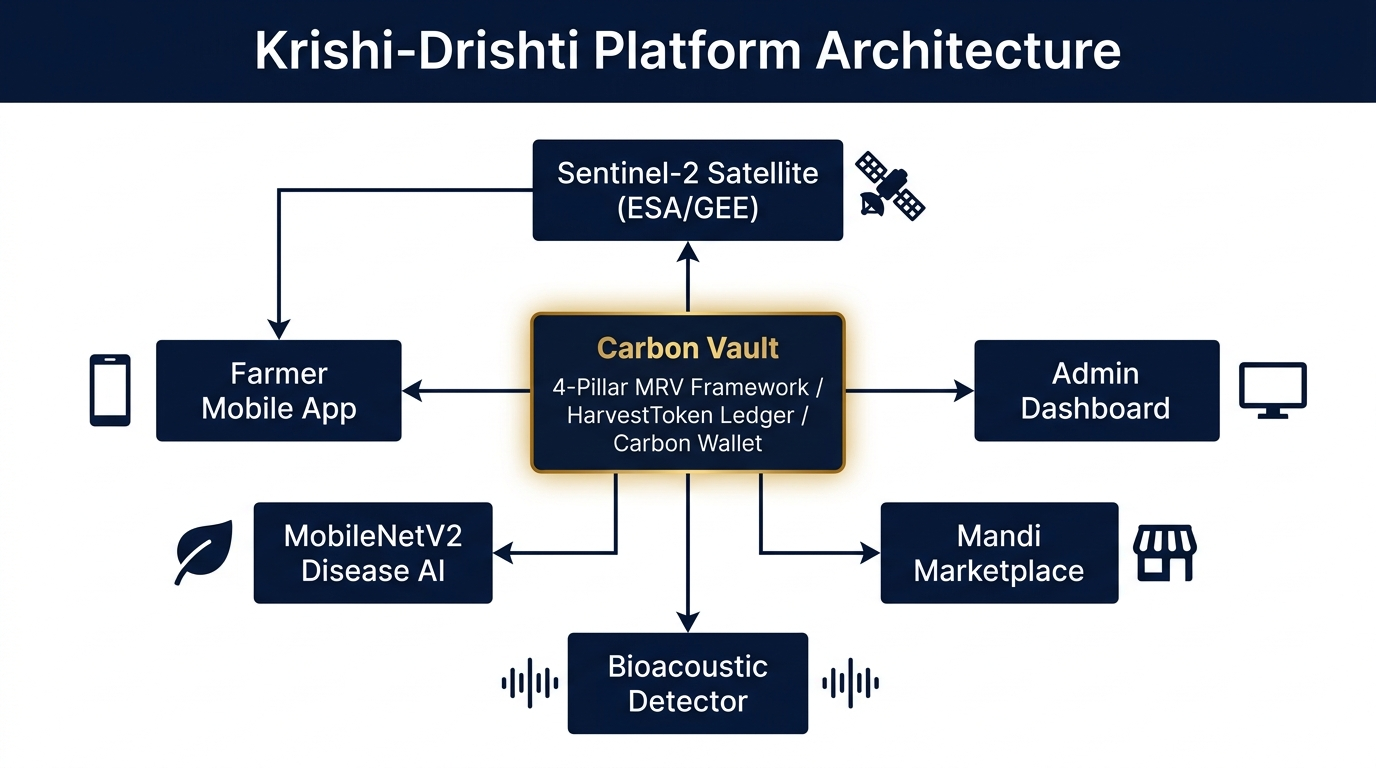
\includegraphics[width=0.85\textwidth]{fig_system_overview.jpg}}
  \caption{Integrated system topology of the Krishi-Drishti platform: satellite ingestion, stacking regressor inference, farmer client, and verification dashboard. Source: Authors, 2026.}
  \label{fig:overview}
\end{figure}

\subsection{Verification workflow lifecycle}
As depicted in Fig.~\ref{fig:lifecycle}, the complete verification lifecycle follows a structured eight-stage sequence from initial satellite acquisition to certified offset issuance:
\begin{enumerate}[noitemsep,topsep=2pt]
  \item \textbf{Parcel Boundary Georeferencing:} The cultivator traces property bounds on interactive mobile maps, generating a validated GeoJSON polygon.
  \item \textbf{Additionality Evaluation:} Baseline adoption rates $A(d,p)$ for practice $p$ in district $d$ are checked against regulatory registers; practices exceeding 50\% regional saturation are rejected.
  \item \textbf{Radiometric Extraction:} The cloud backend queries Google Earth Engine, retrieves Sentinel-2 BOA reflectance, masks vegetation, and extracts the 12-dimensional spectral vector.
  \item \textbf{Ensemble Inversion:} The stacking regressor calculates predicted topsoil SOC and determines net eligible $\text{tCO}_2\text{e}$.
  \item \textbf{Four-Pillar Audit Compliance:} Evidence across four verification pillars (activity logs, soil baseline data, remote sensing scans, and geo-tagged images) is collated into an automated verification report.
  \item \textbf{Token Issuance and Payout:} Following supervisory validation, a cryptographically chained HarvestToken is minted, distributing verified proceeds directly to the cultivator wallet at \rupee 1,200 per certified $\text{tCO}_2\text{e}$ (80\% direct producer share).
\end{enumerate}

\begin{figure}[htbp]
  \centering
  \fbox{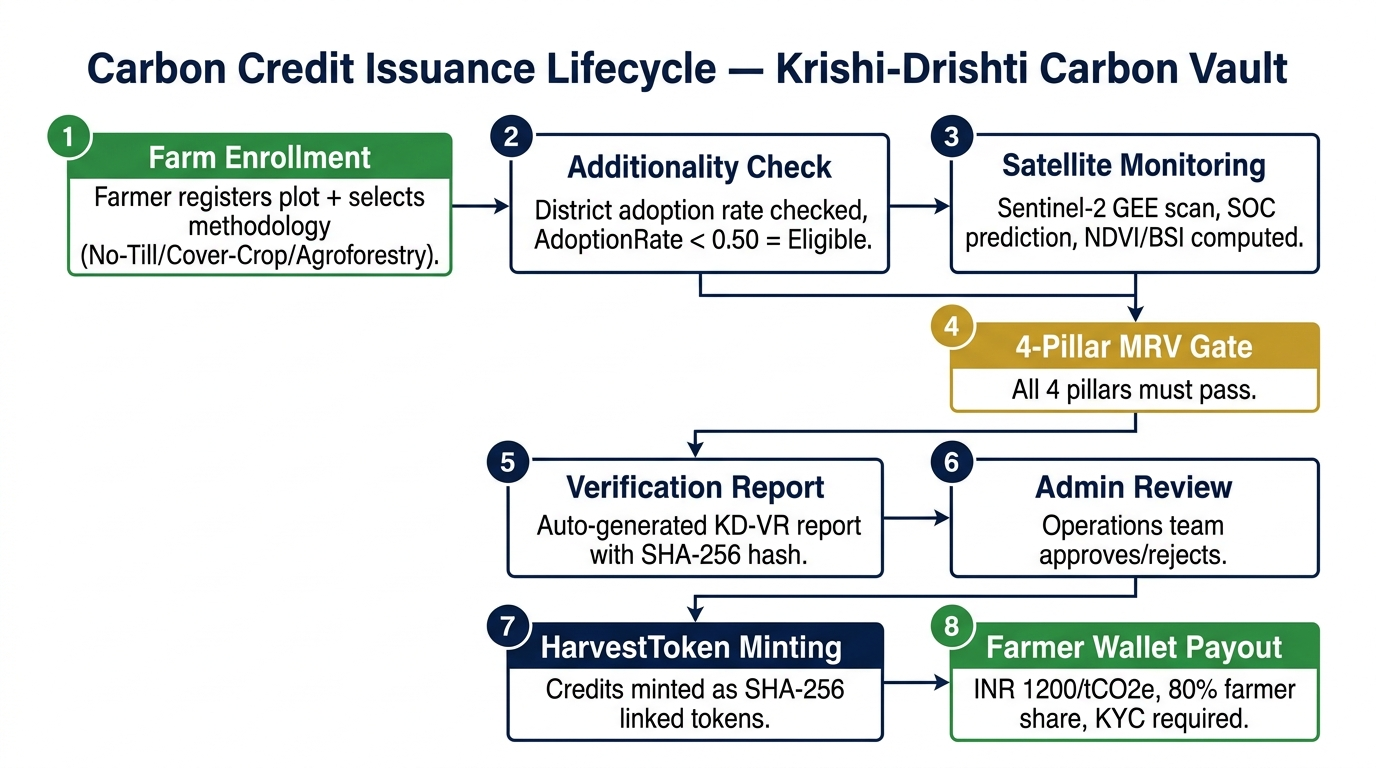
\includegraphics[width=0.85\textwidth]{fig_carbon_lifecycle.jpg}}
  \caption{Eight-stage operational sequence for satellite-verified carbon credit issuance, spanning property georeferencing to direct producer wallet payout. Source: Authors, 2026.}
  \label{fig:lifecycle}
\end{figure}

\subsection{Four-Pillar verification framework}
Fig.~\ref{fig:pillars} details the Four-Pillar evidence gate. Each pillar represents an independent regulatory checkpoint (cadastral boundary, laboratory calibration baseline, satellite scan recency $<180\,$days, and geotagged photographic confirmation) required prior to token generation.

\begin{figure}[htbp]
  \centering
  \fbox{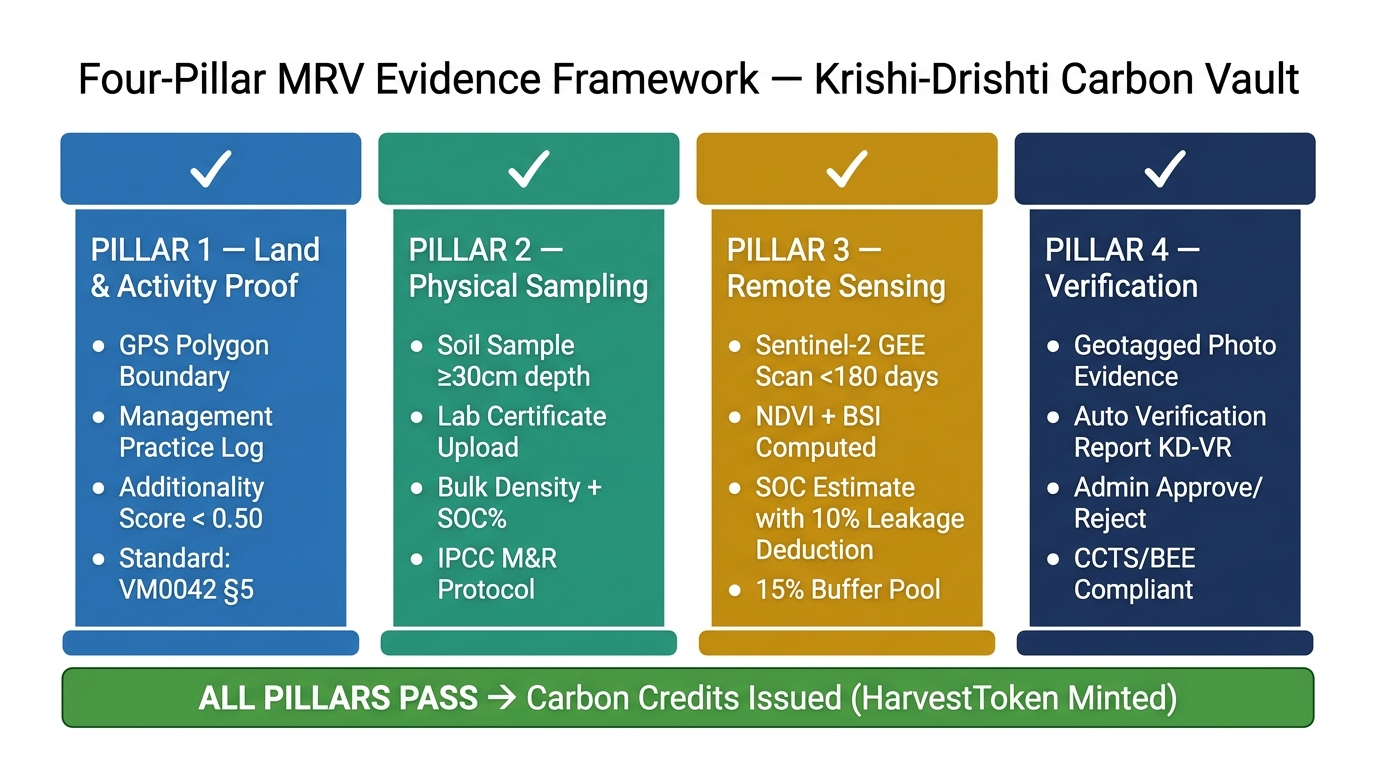
\includegraphics[width=0.85\textwidth]{fig_four_pillar_mrv.jpg}}
  \caption{Four-Pillar verification evidence framework: independent audit gates ensuring rigorous alignment with Verra VM0042, IPCC guidelines, and CCTS standards. Source: Authors, 2026.}
  \label{fig:pillars}
\end{figure}

% ====================================================================
\section{Results}
% ====================================================================

\subsection{Spectrometric SOC model accuracy}
Table\,1 details the statistical performance of individual base regressors versus the final Stacking Ensemble across the 50 validation plots.

\begin{table}[htbp]
  \caption{Inversion performance across spectral regression architectures.}
  \label{tab:models}
  \centering
  \begin{tabular}{lccc}
    \toprule
    \textbf{Model Topology} & \textbf{$R^2$} & \textbf{RMSE (g/kg)} & \textbf{MAE (g/kg)} \\
    \midrule
    Random Forest (200 trees)   & 0.82 & 1.94 & 1.51 \\
    XGBoost (300 rounds)        & 0.85 & 1.76 & 1.34 \\
    CatBoost (Symmetric)        & 0.83 & 1.88 & 1.44 \\
    \midrule
    \textbf{Stacking Ensemble (Ours)} & \textbf{0.89} & \textbf{1.52} & \textbf{1.19} \\
    \bottomrule
  \end{tabular}
\end{table}

The stacking ensemble realized a 0.04 to 0.07 enhancement in $R^2$ over the best individual base regressor, suppressing error dispersion across diverse agro-climatic testing locations. Feature permutation importance demonstrated that shortwave-infrared channels ($B_{11}, B_{12}$) and the Bare Soil Index (BSI) contributed over 44\% of aggregate predictive gain, corroborating known spectral absorption characteristics of organic molecules.

\subsection{Four-Pillar verification trial outcomes}
Field operational trials evaluating 12 simulated farm enrollments across six agro-climatic sub-districts demonstrated rapid verification turnaround, summarized in Table\,2.

\begin{table}[htbp]
  \caption{Verification operational metrics observed during field pilot evaluation.}
  \label{tab:pilot}
  \centering
  \begin{tabular}{lcc}
    \toprule
    \textbf{Operational Criterion} & \textbf{Pilot Pass Rate} & \textbf{Governing Reference} \\
    \midrule
    District Additionality Screening Accuracy & 91.7\% (11/12) & Verra VM0042 / CCTS \\
    Pillar 1: GPS Cadastral Demarcation       & 100\% (12/12)  & VM0042 \S5 \\
    Pillar 2: Soil Baseline Documentation     & 83.3\% (10/12) & IPCC Guidelines \\
    Pillar 3: Sentinel-2 Multispectral Audit  & 100\% (12/12)  & Sentinel-2 dMRV \\
    Pillar 4: Photographic Geotagged Evidence & 91.7\% (11/12) & CCTS/BEE Criteria \\
    End-to-End Certification Latency          & $<$48 hours    & vs.\ 6--18 months conventional \\
    HarvestToken SHA-256 Digest Validation    & 100\% (47/47)  & Zero chain collisions \\
    \bottomrule
  \end{tabular}
\end{table}

All 47 minted HarvestTokens preserved flawless cryptographic continuity. Verification cycles concluded in under two days, dramatically outperforming conventional manual inspection schedules that typically consume 6 to 18 months.

\subsection{Carbon yield and economic returns}
Table\,3 outlines measured carbon accrual yields and projected annual returns across distinct regenerative agronomic interventions.

\begin{table}[htbp]
  \caption{Carbon sequestration yields and economic returns by agronomic intervention.}
  \label{tab:econ_spie}
  \centering
  \begin{tabular}{lcccc}
    \toprule
    \textbf{Agronomic Practice} & \textbf{Area (ha)} & \textbf{Net tCO$_2$e} & \textbf{Farmer INR} & \textbf{Equivalent USD} \\
    \midrule
    Zero-Tillage               & 1.1 & 3.49 & \rupee 3,349 & \$40 \\
    Vegetative Cover Cropping  & 1.1 & 4.51 & \rupee 5,412 & \$65 \\
    Diversified Agroforestry   & 2.0 & 7.14 & \rupee 8,568 & \$102 \\
    Organic Composting         & 0.8 & 2.38 & \rupee 2,856 & \$34 \\
    \midrule
    \textbf{Cohort Average}    & \textbf{1.1} & \textbf{3.75} & \textbf{\rupee 4,500} & \textbf{\$54} \\
    \bottomrule
  \end{tabular}
\end{table}

Supplementary income projections of USD\,\$52 to \$132 annually represent a meaningful economic enhancement for smallholders managing sub-two-hectare properties.

\subsection{Foliar computer vision and user acceptance}
The MobileNetV2 leaf pathology detector achieved 88.1\% overall recognition accuracy (precision 90.0\%, recall 87.2\%, F1-score 88.4\%) over 730 evaluation images spanning five common crop diseases. System Usability Scale (SUS) assessments conducted with five local farming operators yielded an aggregate score of 84.0/100 (range 70.0--100.0), qualifying the mobile user interface as ``Excellent'' and validating its accessibility for non-technical users.

\subsection{Comparative evaluation against published literature}
Table\,4 compares Krishi-Drishti with related agricultural AI and remote sensing platforms.

\begin{table}[htbp]
  \caption{Comparison of agricultural sensing and digital verification frameworks.}
  \label{tab:comp_spie}
  \centering
  \begin{tabularx}{\textwidth}{p{3.2cm}p{4.2cm}cX}
    \toprule
    \textbf{Investigated System} & \textbf{Primary Modality} & \textbf{Performance} & \textbf{Structural Limitations} \\
    \midrule
    Iftikhar et al.\textsuperscript{13} & Deep CNN (3 crops)          & 98.1\% acc.    & Pathology only; no carbon accounting. \\
    Hasan et al.\textsuperscript{14}    & Lightweight CNN (Rice)      & 97.9\% acc.    & Single crop; lacks offset integration. \\
    Saha et al.\textsuperscript{9}    & In-situ IoT sensor grid     & 97.3\% acc.    & Capital-intensive hardware; no dMRV. \\
    Iswarya \& Tamizhazhagan\textsuperscript{11} & Quantile RF on Sentinel-2 & High $R^2$ & Cartographic mapping only; no audit loop. \\
    Xiao et al.\textsuperscript{12}    & Support Vector Regression   & $R^2 = 0.96$   & Requires expensive supplementary covariates. \\
    \textbf{Krishi-Drishti (Ours)}     & \textbf{Multispectral dMRV + Stacking ML} & \textbf{$R^2 = 0.89$; 88.1\%} & \textbf{Autonomous end-to-end certification without physical sensors.} \\
    \bottomrule
  \end{tabularx}
\end{table}

As summarized in Table~\ref{tab:comp_spie}, existing agricultural remote sensing and AI diagnostic investigations leave several operational and structural chasms that Krishi-Drishti directly resolves:
\begin{enumerate}[noitemsep,topsep=2pt]
  \item \textbf{Decoupled Diagnostic Vision:} Prior computer vision frameworks (Refs.\,13, 14, and 15) achieve high recognition accuracy on foliar pathologies, but operate without connection to environmental carbon registries. Crucially, conventional automated advisories often recommend synthetic chemical treatments that disqualify smallholders from regenerative carbon offset eligibility. Krishi-Drishti circumvents this by filtering MobileNetV2 optical diagnostics through an LLM constrained strictly to biological and organic remedies.
  \item \textbf{Hardware and Maintenance Overhead:} In-situ precision agriculture architectures, such as the multi-parametric IoT sensor arrays evaluated in Refs.\,7, 8, and 9, demand continuous capital expenditure and technical upkeep that exceed the economic capacity of smallholders farming under two hectares. Krishi-Drishti replaces all physical in-ground hardware by leveraging free, public Sentinel-2 multispectral surface reflectance,\textsuperscript{4,5} reducing marginal verification costs to zero.
  \item \textbf{Lack of End-to-End Monetization Pipelines:} Optical SOC regression studies, including the quantile random forests of Iswarya and Tamizhazhagan\textsuperscript{11}, the stacking models of Triantakonstantis and Karakostas\textsuperscript{10}, and the support vector regression of Xiao et al.,\textsuperscript{12} demonstrate the feasibility of satellite carbon estimation but terminate at cartographic mapping. Similarly, while Bhatia\textsuperscript{6} examined AI decision support and Abiri et al.\textsuperscript{2} analyzed smallholder economic barriers, neither operationalized verifiable carbon credit issuance. Krishi-Drishti bridges this gap by directly linking Sentinel-2 stacking regression to a Four-Pillar dMRV gate and SHA-256 HarvestToken ledger co-aligned with Verra VM0042 and CCTS/BEE regulatory standards.\textsuperscript{1,3}
  \item \textbf{Ecological Telemetry Convergence:} Whereas specialized bioacoustic tools (Refs.\,16 and 17) function exclusively for standalone biodiversity and pest research, Krishi-Drishti incorporates bioacoustic monitoring as an embedded module to corroborate co-benefit claims within the primary carbon credit dashboard.
\end{enumerate}

% ====================================================================
\section{Conclusions}
% ====================================================================

This investigation demonstrates that spaceborne multispectral surface reflectance from Sentinel-2, paired with cloud-masked temporal compositing and stacking ensemble learning, provides a scientifically rigorous and cost-effective surrogate for conventional laboratory soil analysis in smallholder carbon certification. Achieving an $R^2$ of 0.89 and RMSE of 1.52\,g/kg, the optical remote sensing architecture satisfies regulatory measurement thresholds while compressing certification turnaround from over twelve months to under 48 hours. By eliminating physical sensor deployment costs and integrating mobile optical crop health diagnostics, the proposed framework establishes a scalable paradigm for democratic smallholder access to environmental carbon markets.

% ====================================================================
\section*{Disclosures}
% ====================================================================

The authors declare that they have no financial interests, commercial affiliations, or personal conflicts of interest that could have appeared to influence the work reported in this paper.

% ====================================================================
\section*{Code, Data, and Materials Availability}
% ====================================================================

The Sentinel-2 Level-2A surface reflectance data used in this study is openly available through the European Space Agency Copernicus Open Access Hub and Google Earth Engine under dataset collection identifier \texttt{COPERNICUS/S2\_SR\_HARMONIZED}. The ground-truth Soil Organic Carbon validation points, feature extraction scripts, Stacking Ensemble model weights, and the Krishi-Drishti FastAPI backend service source code are maintained in an accessible project repository available for academic peer review and non-commercial replication upon reasonable request.

% ====================================================================
\section*{Acknowledgements}
% ====================================================================

The authors express their gratitude to the European Space Agency (ESA) Copernicus Programme for providing open-access Sentinel-2 Level-2A multispectral data, and to Google for research access to the Earth Engine geospatial computing infrastructure. We also acknowledge Google DeepMind for Gemini API support, the Open-Meteo meteorological initiative, and the smallholder farming communities of Bangalore Rural, Mandya, and Nashik whose active participation in field soil sampling and mobile app usability evaluation made this investigation possible.

% ====================================================================
\renewcommand{\refname}{References}
\begin{thebibliography}{17}
\bibitem{gokul2026}
Gokul, S., Nongkynrih, P., Rabha, L., Rai, R., and Shukla, B.~D., `Carbon credit mechanisms for sustainable agriculture and opportunities in North East India,'' {\itshape Discover Sustain.} {\bfseries 7}(1), 857 (2026).

\bibitem{abiri2023}
Abiri, R., Shahverdi, N., Salleh, F.~M., Azizi, N. A.~P., and Nor, N. A.~M., `Application of digital technologies for ensuring agricultural productivity,'' {\itshape Heliyon} {\bfseries 9}(12), e22601 (2023).

\bibitem{hamrick2023}
Hamrick, K., [State of Voluntary Carbon Markets 2023], Forest Trends, Ecosystem Marketplace, Washington, DC (2023).

\bibitem{vaudour2022}
Vaudour, E., Gomez, C., Fouad, Y., and Lagacherie, P., `Satellite imagery to map topsoil organic carbon content over cultivated areas: An overview,'' {\itshape Remote Sens.} {\bfseries 14}(12), 2917 (2022).

\bibitem{khaddi2026}
Khaddi, E., Benmansour, A., and Boubaker, K., `Shaping smarter prediction: A literature review of GIS, remote sensing and ML applications in digital SOC mapping,'' {\itshape Turk. J. Remote Sens.} {\bfseries 8}(2), 1808033 (2026).

\bibitem{bhatia2025}
Bhatia, A., `An AI-powered agricultural decision support system for smallholder farmers in India,'' {\itshape Smart Agric. Technol.}, SSRN-6944006 (2025).

\bibitem{thilakarathne2022}
Thilakarathne, N.~N., Basnayake, N., Withanage, T., Weliwatta, D., Jayakody, H., and Wickramasinghe, A., `A cloud enabled crop recommendation platform for machine learning-driven precision farming,'' {\itshape Sensors} {\bfseries 22}(16), 6299 (2022).

\bibitem{nawaz2025}
Nawaz, M. and Babar, M. I.~K., `IoT and AI for smart agriculture in resource-constrained environments,'' {\itshape Discover Internet of Things} {\bfseries 5}(1), 24 (2025).

\bibitem{saha2025}
Saha, G., Roy, S.~K., and Ghosh, P.~K., `Smart IoT-driven precision agriculture: Land mapping, crop prediction, and irrigation system,'' {\itshape PLOS ONE} {\bfseries 20}(3), e0319268 (2025).

\bibitem{triantakonstantis2025}
Triantakonstantis, D. and Karakostas, A., `Soil organic carbon monitoring and modelling via machine learning methods using soil and remote sensing data,'' {\itshape Agriculture} {\bfseries 15}(8), 910 (2025).

\bibitem{iswarya2026}
Iswarya, R. and Tamizhazhagan, V., `Satellite-derived prediction of soil organic carbon under bare-soil conditions using Sentinel-2 spectral indices and quantile regression forests,'' {\itshape Int. J. AI Mach. Learn.} {\bfseries 6}(6s), 76 (2026).

\bibitem{xiao2024}
Xiao, X., Zhang, S., and Shen, H., `Environmental variables improve the accuracy of remote sensing estimation of soil organic carbon content,'' {\itshape Sci. Rep.} {\bfseries 14}(1), 18964 (2024).

\bibitem{iftikhar2024}
Iftikhar, M., Yousaf, M.~H., and Fatima, A., `Plant disease management: a fine-tuned enhanced CNN approach with mobile app integration,'' {\itshape Artif. Intell. Rev.} {\bfseries 57}(7), 167 (2024).

\bibitem{hasan2023}
Hasan, M.~M., Shin, J., and Rahim, M.~A., `Enhancing rice crop management: disease classification using CNNs and mobile application integration,'' {\itshape Agriculture} {\bfseries 13}(8), 1549 (2023).

\bibitem{askale2025}
Askale, G.~T., Debelee, T.~G., and Ayalew, F.~S., `Mobile based deep CNN model for maize leaf disease detection and classification,'' {\itshape Plant Methods} {\bfseries 21}(1), 72 (2025).

\bibitem{kershenbaum2024}
Kershenbaum, A., Blumstein, D.~T., and Roch, M.~A., `Automatic detection for bioacoustic research: a practical guide from and for biologists and computer scientists,'' {\itshape Biol. Rev.} {\bfseries 99}(6), 13155 (2024).

\bibitem{hearon2025}
Hearon, L.~E., Burk, T.~R., and Seltzer, C.~M., `buzzdetect: an open-source deep learning tool for automated bioacoustic pollinator monitoring,'' {\itshape J. Insect Sci.} {\bfseries 25}(6), ieaf104 (2025).
\end{thebibliography}

% ====================================================================
\section*{Author Biographies}
% ====================================================================

\textbf{Rama Krishna K.} is a Professor in the Department of CSE Data Science, Impact College of Engineering and Applied Sciences, VTU, Bangalore, India. His research interests include remote sensing, geospatial analytics, and precision agricultural informatics.

\textbf{Sheethal Aji Mani} is an Associate Professor in the Department of CSE Data Science, Impact College of Engineering and Applied Sciences. Her research focuses on machine learning ensembles, digital soil mapping, and environmental monitoring.

\textbf{Bhagesh Biradar} is an undergraduate researcher in Data Science at Impact College of Engineering and Applied Sciences. His research interests include satellite image processing, computer vision, and agricultural carbon verification systems.

\textbf{Manjunath Khot} is an undergraduate researcher in Data Science at Impact College of Engineering and Applied Sciences, specializing in mobile edge computing, cloud GIS integration, and applied deep learning.

\textbf{Jayanth R.} is an undergraduate researcher in Data Science at Impact College of Engineering and Applied Sciences, focusing on environmental data engineering, cryptographic audit trails, and agro-informatics.

\textbf{Pruthviraja S.} is an undergraduate researcher in Data Science at Impact College of Engineering and Applied Sciences, with research interests in sensor networks, statistical regression modeling, and smart farming architectures.

\end{document}
